%	This LaTeX file is written by Zhiyang Ong as a template for creating presentation slides.

%	The MIT License (MIT)

%	Copyright (c) <2015> <Zhiyang Ong>

%	Permission is hereby granted, free of charge, to any person obtaining a copy of this software and associated documentation files (the "Software"), to deal in the Software without restriction, including without limitation the rights to use, copy, modify, merge, publish, distribute, sublicense, and/or sell copies of the Software, and to permit persons to whom the Software is furnished to do so, subject to the following conditions:

%	The above copyright notice and this permission notice shall be included in all copies or substantial portions of the Software.

%	THE SOFTWARE IS PROVIDED "AS IS", WITHOUT WARRANTY OF ANY KIND, EXPRESS OR IMPLIED, INCLUDING BUT NOT LIMITED TO THE WARRANTIES OF MERCHANTABILITY, FITNESS FOR A PARTICULAR PURPOSE AND NONINFRINGEMENT. IN NO EVENT SHALL THE AUTHORS OR COPYRIGHT HOLDERS BE LIABLE FOR ANY CLAIM, DAMAGES OR OTHER LIABILITY, WHETHER IN AN ACTION OF CONTRACT, TORT OR OTHERWISE, ARISING FROM, OUT OF OR IN CONNECTION WITH THE SOFTWARE OR THE USE OR OTHER DEALINGS IN THE SOFTWARE.

%	Email address: echo "cukj -wb- 23wU4X5M589 TROJANS cqkH wiuz2y 0f Mw Stanford" | awk '{ sub("23wU4X5M589","F.d_c_b. ") sub("Stanford","d0mA1n"); print $5, $2, $8; for (i=1; i<=1; i++) print "6\b"; print $9, $7, $6 }' | sed y/kqcbuHwM62z/gnotrzadqmC/ | tr 'q' ' ' | tr -d [:cntrl:] | tr -d 'ir' | tr y "\n"



%%%%%%%%%%%%%%%%%%%%%%%%%%%%%%%%%%%%%%%%%%%%%%
%	Preamble

%	Acknowledgement:
%		This is based on a template provided to me by Dott. Francesco Stefanni, from the University of Verona in January 2011.
%
%	Number the slides per section. This makes it easier to track the index of the slides (or number of slides) per section, as opposed to the cumulative number of slides. When I manually track the number of slides for a presentation, each time I refactor the set of slides, I would have to update the slide numbers. I want the computer to do this automatically. Hence, I shall not do this manually.



%	Use the Beamer package to create the presentation slides.
\documentclass[xcolor={usenames,dvipsnames},hyperref={hyperindex,bookmarks}]{beamer}


%%%%%%%%%%%%%%%%%%%%%%%%%%%%%%%%%%%%%%%%%%%%%%
%	Import and Customize LaTeX packages.
\usepackage{beamerthemesplit}


%	Package for typesetting the following symbol: $\mathfrak{S}$
%\usepackage{amssymb}

%\mode<presentation>
%{ \usetheme{boxes} }

%	Select the presentation mode.
\mode<presentation>{
	\usetheme[logos=true,pagenumbers=true,background=true]{Esd}
}
\setbeamercovered{transparent}
%\setbeamercovered{invisible}


%	Import package to facilitate typesetting of algorithms.
\usepackage{listings}

\lstset{
  language=C++,
  tabsize=4,
%  basicstyle=\ttfamily\color{black}\small,
  basicstyle=\ttfamily\color{black},
%  backgroundcolor=\color{lightgray},
%  backgroundcolor=\color{white},
  keywordstyle=\color{Purple}\bfseries,
  identifierstyle=\color{OliveGreen},
  commentstyle=\color{Gray}\itshape,
  stringstyle=\color{CarnationPink},
  showstringspaces=false,
  showtabs=false,
  showspaces=false
}


\definecolor{lightgray}{gray}{0.95}
\font\emailtt=cmtt9

%	Set up configuration for hyperlinks.
%\usepackage[pdftex]{hyperref}	-- Option clash
\hypersetup{
    pdftitle={{\it PULPino} attack scenarios},     % title
    pdfauthor={Zhiyang Ong},                 % author
    pdfsubject={Hack@DAC 2018 Contest}, % subject of the document
    pdfcreator={Creator},                           % creator of the document
    pdfproducer={dvipdft},                          % producer of the document
% Modified by Zhiyang Ong on Feb 7, 2011 to improve the way hyperlinks are colored in these presentation slides
	pdfkeywords={LaTeX, graphics, color},
%    pdfkeywords={C, C++, programming style},        % list of keywords
%
%    bookmarks=true,         % show bookmarks bar?
    unicode=false,          % non-Latin characters in Acrobats bookmarks
    pdftoolbar=true,        % show Acrobats toolbar?
    pdfmenubar=true,        % show Acrobats menu?
    pdffitwindow=false,     % window fit to page when opened
% Modified by Zhiyang Ong on Feb 7, 2011 to improve the way hyperlinks are colored in these presentation slides
	pdfpagemode=UseOutlines,bookmarks, bookmarksopen,
	pdfstartview=FitH, colorlinks, linkcolor=blue, citecolor=blue, urlcolor=red,
%    pdfstartview={Fit},    % fits the width of the page to the window
    pdfnewwindow=true,      % links in new window
% Modified by Zhiyang Ong on Feb 7, 2011 to improve the way hyperlinks are colored in these presentation slides
	colorlinks=red,        % false: boxed links; true: colored links
	linkcolor=red,          % color of internal links
%    colorlinks=false,        % false: boxed links; true: colored links
%    linkcolor=red,          % color of internal links
    citecolor=green,        % color of links to bibliography
    filecolor=magenta,      % color of file links
    urlcolor=red,           % color of external links
    pdfpagemode=FullScreen
    %
    %pdfpagelabels=false
}

%\usepackage[all]{hypcap}




%%%%%%%%%%%%%%%%%%%%%%%%%%%%%%%%%%%%%%%%%%%%%%
%	Added by Zhiyang Ong on Feb 7, 2011 to allow figures to be places side-by-side
%\usepackage{subfigure}


%	First slide of the presentation
\title[{DeepSF}]
{\huge 
%{DeepSF}}
{DeepSF}: Deep CNN for mapping protein sequences to folds}
%{DeepSF}: deep convolutional neural network for mapping protein sequences to folds}
\subtitle{Zhiyang's presentation about \cite{Hou2018}}
\author{Zhiyang Ong}
\institute{
	Department of Electrical and Computer Engineering \\
	Dwight Look College of Engineering,\\
	Texas A\&M University \\
	College Station, TX
}
\date{\today}	% (optional)
\subject{Subject Title}







%%%%%%%%%%%%%%%%%%%%%%%%%%%%%%%%%%%%%%%%%%%%%%
%	Do nothing in this section of the LaTeX document

\begin{document}





\begin{frame}
\titlepage
\end{frame}



%	Table of Contents
\AtBeginSection[]		% Do nothing for \subsection*
{
	\begin{frame}
%		\frametitle{\textcolor{yellow}{Table of Contents}}
		\frametitle{Table of Contents}
%		\textcolor{yellow}{\tableofcontents[currentsection]}
		\tableofcontents[currentsection,currentsubsection]
	\end{frame}
}

\AtBeginSubsection[]		% Do nothing for \subsection*
{
\begin{frame}
\tableofcontents[currentsection,currentsubsection]
\end{frame}
}

\section*{Outline}
\begin{frame}
\tableofcontents
\end{frame}



%%%%%%%%%%%%%%%%%%%%%%%%%%%%%%%%%%%%%%%%%%%%%%
%
%	Slides begin HERE!!!
%
%%%%%%%%%%%%%%%%%%%%%%%%%%%%%%%%%%%%%%%%%%%%%%


%%%%%%%%%%%%%%%%%%%%%%%%%%%%%%%%%%%%%%%%%%%%%%
%	Problem and Knowledge Gap

\section{Problem and Knowledge Gap}



%	Slide #1
\frame
{
	\frametitle{Context of the Problem}
	\framesubtitle{Background Information}

	Context of the problem.
	\begin{enumerate}
	\item The structures of most ($>99\%$) proteins are unknown % (pp. 1296, left column, paragraph 1)
	\item Protein fold recognition enables us to associate a protein sequence to a protein fold
		\begin{itemize}	% (pp. 1296, left column, paragraph 1)
		\item Identifying protein homologs that share the same protein fold
		\item With this protein fold, determine its protein structure $[$Tramontano2003$]$
		\item With this protein structure, determine its protein function	%	{\Huge Insert References!!!}
			\begin{itemize}
			\item $[$Osadchy2011,OConnor2010,Tramontano2003,Hegyi1999$]$
			\item $[$OConnor2014a, \href{https://www.nature.com/scitable/ebooks/cell-biology-for-seminars-14760004/122995569/}{From Contents: Unit 2, How Do Cells Decode Genetic Information into Functional Proteins?: \S2.4 The Functions of Proteins Are Determined by Their Three-Dimensional Structures}$]$
			\item $[$OConnor2014, \href{ https://www.nature.com/scitable/ebooks/essentials-of-cell-biology-14749010/122996920/}{From Contents: Unit 2, How Do Cells Decode Genetic Information into Functional Proteins?: \S2.4 The Functions of Proteins Are Determined by Their Three-Dimensional Structures}$]$
			\end{itemize}
		\end{itemize}
	\end{enumerate}

%Other resources:
%+ https://socratic.org/questions/what-is-the-relationship-between-a-protein-s-structure-and-its-ability-to-functi


}


%Resources for background information:
%+ https://en.wikipedia.org/wiki/Bioinformatics
%+ https://en.wikipedia.org/wiki/Structural_bioinformatics
%+ https://en.wikipedia.org/wiki/Sequence_homology
%+ https://en.wikipedia.org/wiki/Structural_genomics
%+ https://en.wikipedia.org/wiki/Protein_structure_prediction
%	``[protein structure prediction is] the inverse problem of protein design''
%	``Protein structure prediction is one of the most important goals pursued by bioinformatics and theoretical chemistry; it is highly important in medicine (for example, in drug design) and biotechnology (for example, in the design of novel enzymes).''
%	https://en.wikipedia.org/wiki/Drug_design
%+ https://en.wikipedia.org/wiki/Functional_genomics
%+ https://en.wikipedia.org/wiki/Genomics
%+ https://en.wikipedia.org/wiki/Biotechnology







%	Slide #2
\frame
{
	\frametitle{Problem Definition - 1}
	\framesubtitle{What is the problem that \cite{Hou2018} is solving?}

	Problem description...
	\begin{enumerate}
	\item Problems with sequence-based methods, especially sequence alignment methods (including profile-sequence and profile-profile alignment methods)  % (abstract, pp. 1296, left column, 2nd paragraph)
		\begin{itemize}
		\item Methods for mapping protein sequences to protein folds are indirect
		\item Can't explain relationship between protein sequences \& protein folds, even machine learning (ML) methods
		\item traditional ML methods also can't work for classifying data into large number of categories ($>1000$)
			% (pp. 1296, left column, 3rd paragraph)
			\begin{itemize}
			\item multi-layer perceptron
			\item support-vector machines
			\item ensemble classifiers
			\item kernel-based learning
			\end{itemize}
		\end{itemize}
	\item Other methods have methodological limitations % abstract
	\end{enumerate}

%Other resources:
%+ https://socratic.org/questions/what-is-the-relationship-between-a-protein-s-structure-and-its-ability-to-functi
}




%	Slide #3
\frame
{
	\frametitle{Problem Definition - 2}
	\framesubtitle{What is the problem that \cite{Hou2018} is solving?}

	Problem description... Continued.
	\begin{enumerate}
	\item Protein fold recognition enables us to associate a protein sequence to a protein fold
		\begin{itemize}	% (pp. 1296, left column, paragraph 1)
		\item With this protein fold, we can determine its protein structure
		\item With this protein structure, we can determine its protein function
		\end{itemize}
	\end{enumerate}
	
	Specifically... Solve the protein fold recognition problem.
	\begin{enumerate}
	\item Given a protein sequence, map it to a protein fold {\bf directly}
	\item Explain relationship between protein sequences \& protein folds
	\end{enumerate}
	

%Other resources:
%+ https://socratic.org/questions/what-is-the-relationship-between-a-protein-s-structure-and-its-ability-to-functi
}




%	Slide #2
\frame
{
	\frametitle{Problem Importance}
	\framesubtitle{Why is it important?}


	Why is this problem important?
	\begin{itemize}
	\item This facilitates protein structure prediction
	\item Knowing about protein folds help us in protein structure prediction
	\item Protein structure prediction enables protein function prediction
	\item Knowing about protein structure and function facilitates:
			\begin{itemize}
			\item drug/medication design $[$Nogrady2005, \S1.6.4, pp. 54$]$ $[$Golan2008, Chapter 1, pp. 4$]$
				% \cite[\S1.6.4, pp. 54]{Nogrady2005}, application of quantum pharmacology to macromolecular modeling to perform protein structure prediction
				% \cite[Chapter 1, pp. 4]{Golan2008}, conformation and chemistry of drugs and receptors, human and microbial drug receptors
			\item biotechnology $[$Walsh2014, Chapter 2$]$
				% \cite[Chapter 2]{Walsh2014}
			\item synthetic biology $[$Zhao2013d, Chapter 2$]$
			\item personalized $[$Cullis2015, Chapter 2, pp. 26$]$ or precision medicine $[$Mousa2020, \S24.3.2, pp. 778$]$
				% \cite[Chapter 2, pp. 26]{Cullis2015}, protein structure determines how we differ from other people
				% \cite[S24.3.2]{}, immune system is affected abiotically by protein structure
			\item gene therapy $[$Wecker2010, Chapter 5, pp. 51$]$
			\end{itemize}
	\end{itemize}
}




%	protein structure prediction
%+ DOI:10.1109/ICBBT.2010.5479021
%+ DOI:10.1038/nbt.2419
%+ DOI:10.1007/978-3-319-41279-5_7
%	structure-based methods for protein function prediction, but did not mention anything about the relationship between them or mention it


%Prediction of Protein Structures, Functions, and Interactions
%	https://www.google.com/books/edition/Prediction_of_Protein_Structures_Functio/VWJDuuF5hsgC?hl=en&gbpv=0

%	https://books.google.com/books?hl=en&lr=&id=LeRhAoz4NwEC&oi=fnd&pg=PA1&dq=%22protein+structure+prediction%22+survey&ots=yB8g0y4JO2&sig=l-SZkUY2PO525v88x1WrXbP4wT0#v=onepage&q=%22protein%20structure%20prediction%22%20survey&f=false
%	https://www.google.com/books/edition/Introduction_to_Protein_Structure_Predic/LeRhAoz4NwEC?hl=en&gbpv=1&dq=%22protein+structure+prediction%22&printsec=frontcover
%	https://www.google.com/books/edition/Introduction_to_Protein_Structure_Predic/5WnNjwEACAAJ?hl=en
%	https://www.google.com/books/edition/Protein_Structure_Prediction/C6XgZJRrFsYC?hl=en&gbpv=1&dq=%22protein+structure+prediction%22&printsec=frontcover
%	https://www.google.com/books/edition/Protein_Folding_in_Silico/9XRHAgAAQBAJ?hl=en&gbpv=1&dq=%22protein+structure+prediction%22&printsec=frontcover
%	https://www.google.com/books/edition/Prediction_of_Protein_Structures_Functio/VWJDuuF5hsgC?hl=en&gbpv=1&dq=%22protein+structure+prediction%22&printsec=frontcover
%	https://www.google.com/books/edition/Protein_Structure_Prediction/7qnvvQAACAAJ?hl=en
%	https://link.springer.com/search?query=%22Protein+Structure+Prediction%22&facet-content-type=%22Book%22
%		https://link.springer.com/book/10.1007/978-1-4939-0366-5 (not a textbook)
%https://link.springer.com/book/10.1007/978-1-59745-574-9
%https://link.springer.com/book/10.1007/978-1-59745-574-9

%https://www.google.com/books/edition/Protein_Structure_Prediction/C6XgZJRrFsYC?hl=en&gbpv=0
%https://www.google.com/books/edition/Protein_Structure_Prediction/7qnvvQAACAAJ?hl=en

%	https://www.google.com/books/edition/Protein_Structure/-DxTZ8ufPzQC?hl=en&gbpv=1&dq=%22protein+function%22+%22drug+design%22&printsec=frontcover
%		https://www.taylorfrancis.com/books/9780429213564
%		https://www.crcpress.com/Protein-Structure-Determination-Analysis-and-Applications-for-Drug-Discovery/author/p/book/9780203911327

%	https://www.google.com/books/edition/Introduction_to_Proteins/-4ZXDwAAQBAJ?hl=en&gbpv=1&dq=%22protein+function%22+%22drug+design%22&printsec=frontcover


%	https://www.google.com/books/edition/Protein_Engineering_and_Design/ycVoWFqDTmAC?hl=en&gbpv=1&dq=pharmacology+%22protein+structure%22&printsec=frontcover



%	https://books.google.com/books?id=EkxCWOoYB2wC&newbks=0&printsec=frontcover&pg=PA54&dq=pharmacology+%22protein+structure%22&hl=en&source=newbks_fb#v=onepage&q=pharmacology%20%22protein%20structure%22&f=false
%		application of quantum pharmacology to macromolecular modeling to perform protein structure prediction
%	\S1.6.4, pp. 54


%https://www.google.com/books/edition/Encyclopedia_of_Molecular_Pharmacology/iwwo5gx8aX8C?hl=en&gbpv=1&kptab=overview
%https://link.springer.com/referencework/10.1007%2F978-3-540-38918-7


%https://www.google.com/books/edition/Pharmacology_of_G_Protein_Coupled_Recept/nP7sGtuaRBEC?hl=en&gbpv=0&kptab=getbook
%https://www.elsevier.com/books/pharmacology-of-g-protein-coupled-receptors/enna/978-0-12-385952-5
%https://www.amazon.com/s?k=9780123859532&i=stripbooks&linkCode=qs


%https://www.ncbi.nlm.nih.gov/pmc/articles/PMC4671355/
%https://www.frontiersin.org/articles/10.3389/fcvm.2015.00014/full



%	Slide #3
\frame
{
	\frametitle{What are the Knowledge Gaps in \cite{Hou2018}?}
	\framesubtitle{How would \cite{Hou2018} address these knowledge gaps?}

	List of knowledge gaps:
	\begin{itemize}
	\item Lack of direct methods for mapping protein sequences to protein folds
	\item Methods can't explain relationship between protein sequences \& protein folds
	\end{itemize}

}
























%%%%%%%%%%%%%%%%%%%%%%%%%%%%%%%%%%%%%%%%%%%%%%
%	Proposed Solution(s)

\section{Proposed Solution(s)}


%	Slide #1
\frame
{
	\frametitle{Proposed Solution(s) - 1}
	\framesubtitle{What do they proposed to address the knowledge gap?}

	Proposed Solution(s).
	\begin{itemize}
	\item Use 1-D deep convolutional neural network (deep CNN) 
	\end{itemize}
}










%	Slide #2
\frame
{
	\frametitle{Proposed Solution(s) - 2}
	\framesubtitle{What do they proposed to address the knowledge gap?}

	Proposed Solution(s).
	\begin{itemize}
	\item Use input feature generation and label assignment from PSI-BLAST.
	\item Specifically, use position-specific scoring matrix
	\item Train all mini-batches for 100 epochs
	\item Distance metrics
		\begin{enumerate} 
		\item Euclid-D, Euclidean distance
		\item Manh-D, Manhattan distance
		\item Corr-D, Pearson's Correlation score
		\item KL-D, KL-Divergence
		\end{enumerate}
	\end{itemize}
}







%	Slide #3
\frame
{
	\frametitle{Proposed Solution(s) - 3}
	\framesubtitle{Architecture for a 1-D deep CNN}


	\begin{figure}[h]
	\centering 
	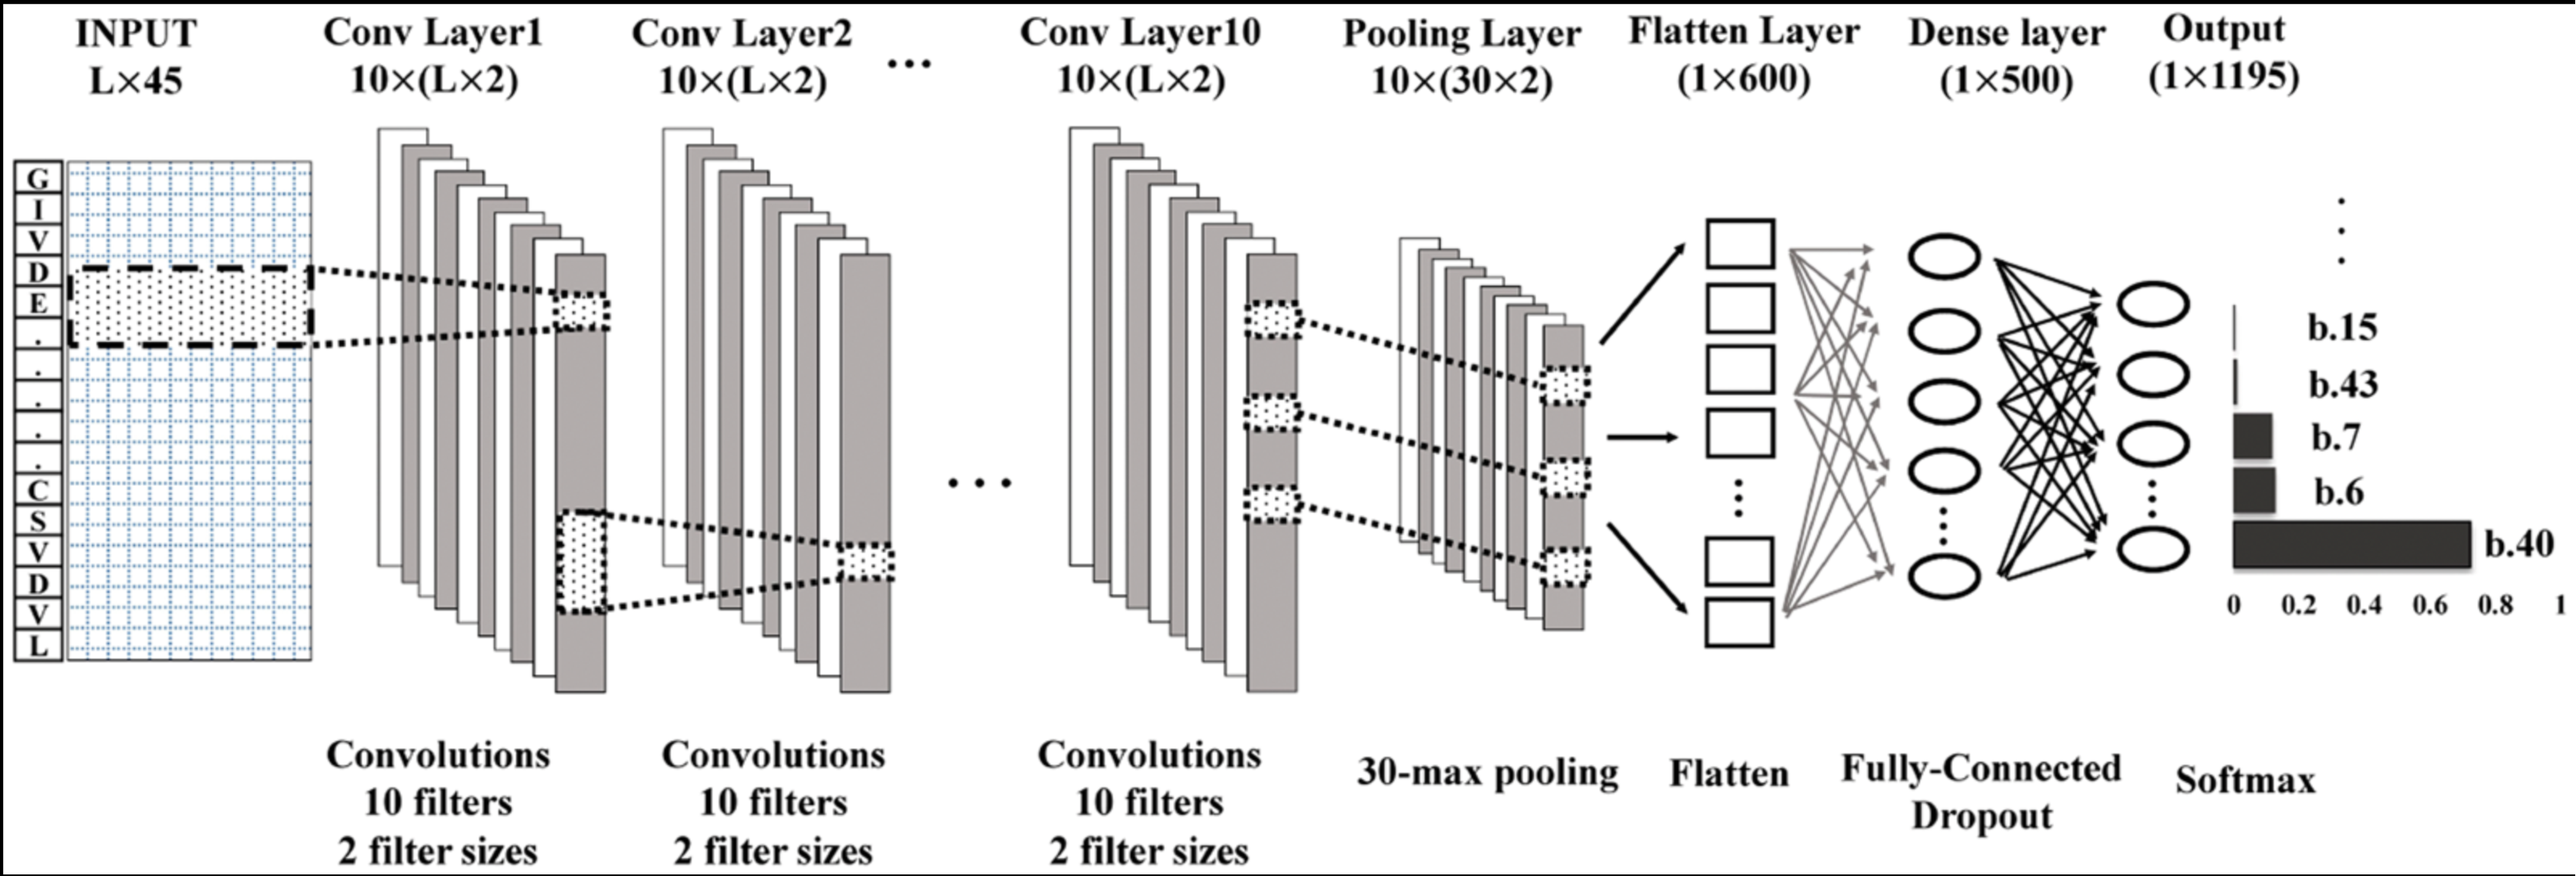
\includegraphics[height=1.5in]{./pics/1-d-cnn-architecture}
	%\caption{The prediction accuracy at family/superfamily/fold levels for top 1, top 5 and top 10 predictions of DeepSF and PSI-BLAST, on SCOP 1.75 test dataset}
	\label{fig:1DdeepCNNarch}
	\end{figure}
}









%	Slide #3
\frame
{
	\frametitle{Dataset and Methods}
	\framesubtitle{Which datasets were used?}

	\begin{itemize}
	\item SCOP 1.75 was used for training and validation (\S3.1)
	\item SCOP 2.06 (\S3.2) and CASP (\S3.3) was used for test
	\end{itemize}
}













%%%%%%%%%%%%%%%%%%%%%%%%%%%%%%%%%%%%%%%%%%%%%%
%	Experimental Results

\section{Experimental Results}



%	Slide #1
\frame
{
	\frametitle{Experimental Results - 1}
	\framesubtitle{Evaluation of distance metrics based on clustering accuracy}


	\begin{figure}[h]
	\centering 
	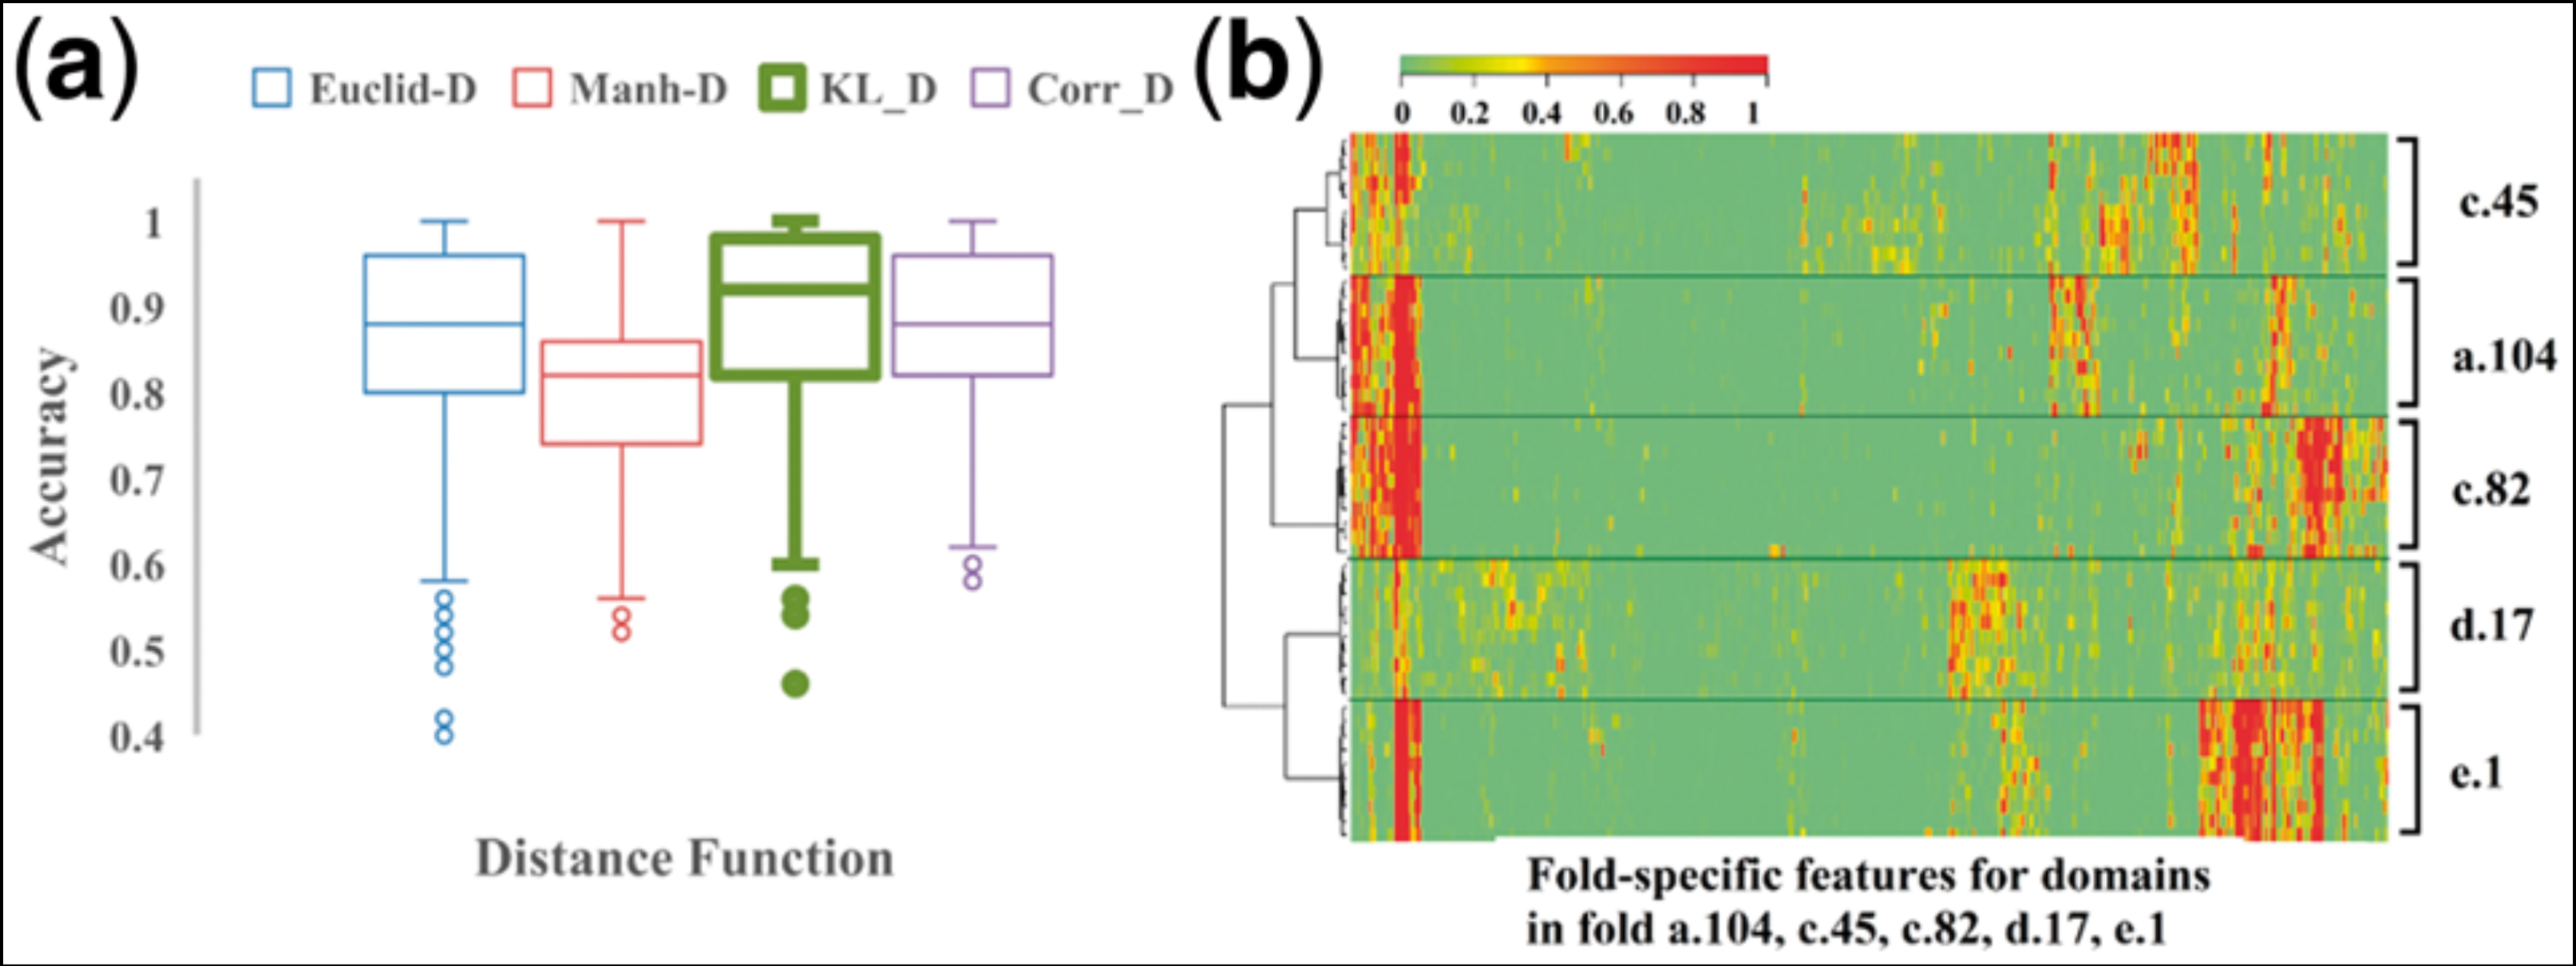
\includegraphics[height=1.6in]{./pics/distance-metrics}
	\caption{The prediction accuracy at family/superfamily/fold levels for top 1, top 5 and top 10 predictions of DeepSF and PSI-BLAST, on SCOP 1.75 test dataset}
	\label{fig:distancemetrics}
	\end{figure}
}








%	Slide #1
\frame
{
	\frametitle{Experimental Results - 1}
	\framesubtitle{How do their proposed solutions compare with existing solutions?}


	\begin{figure}[h]
	\centering 
	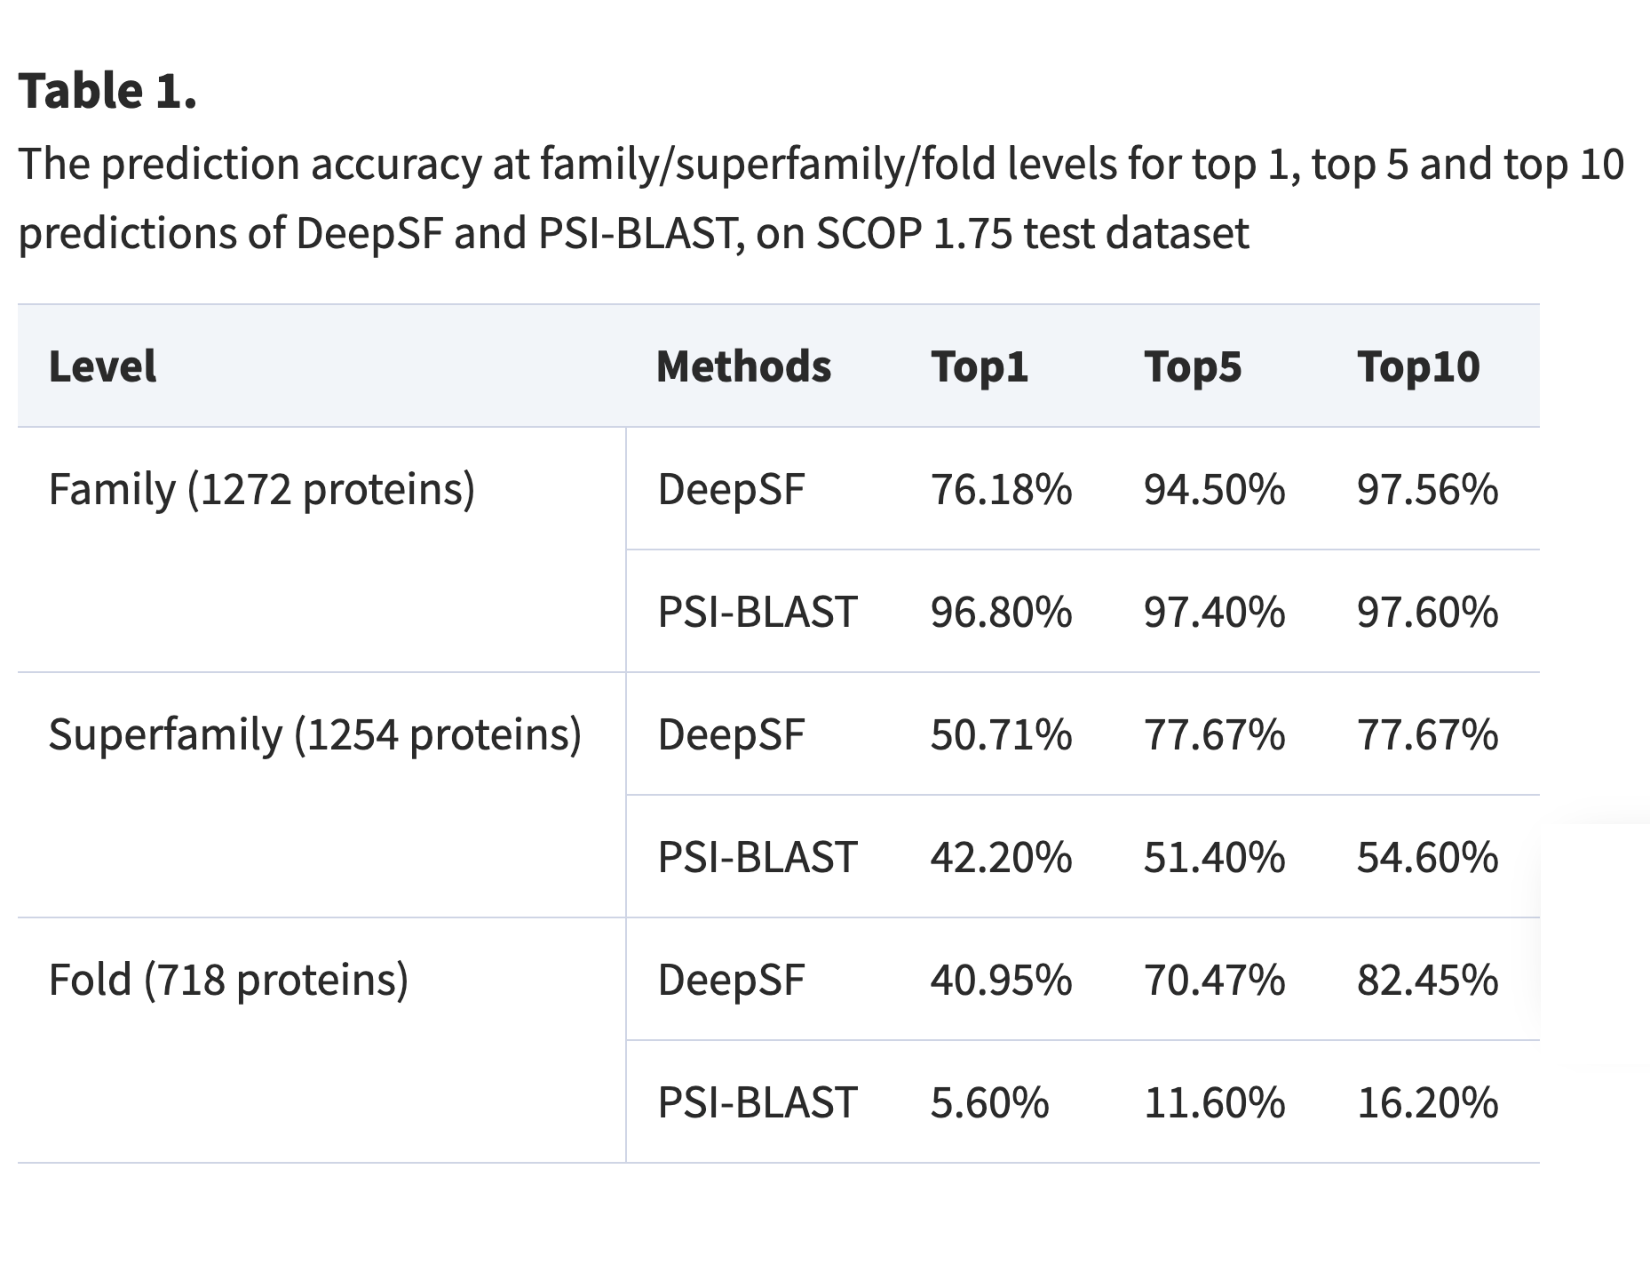
\includegraphics[height=2.5in]{./pics/table-1}
	%\caption{The prediction accuracy at family/superfamily/fold levels for top 1, top 5 and top 10 predictions of DeepSF and PSI-BLAST, on SCOP 1.75 test dataset}
	\label{fig:Table1}
	\end{figure}
}




%	Slide #2
\frame
{
	\frametitle{Experimental Results - 2}
	\framesubtitle{How do their proposed solutions compare with existing solutions?}


	\begin{figure}[h]
	\centering 
	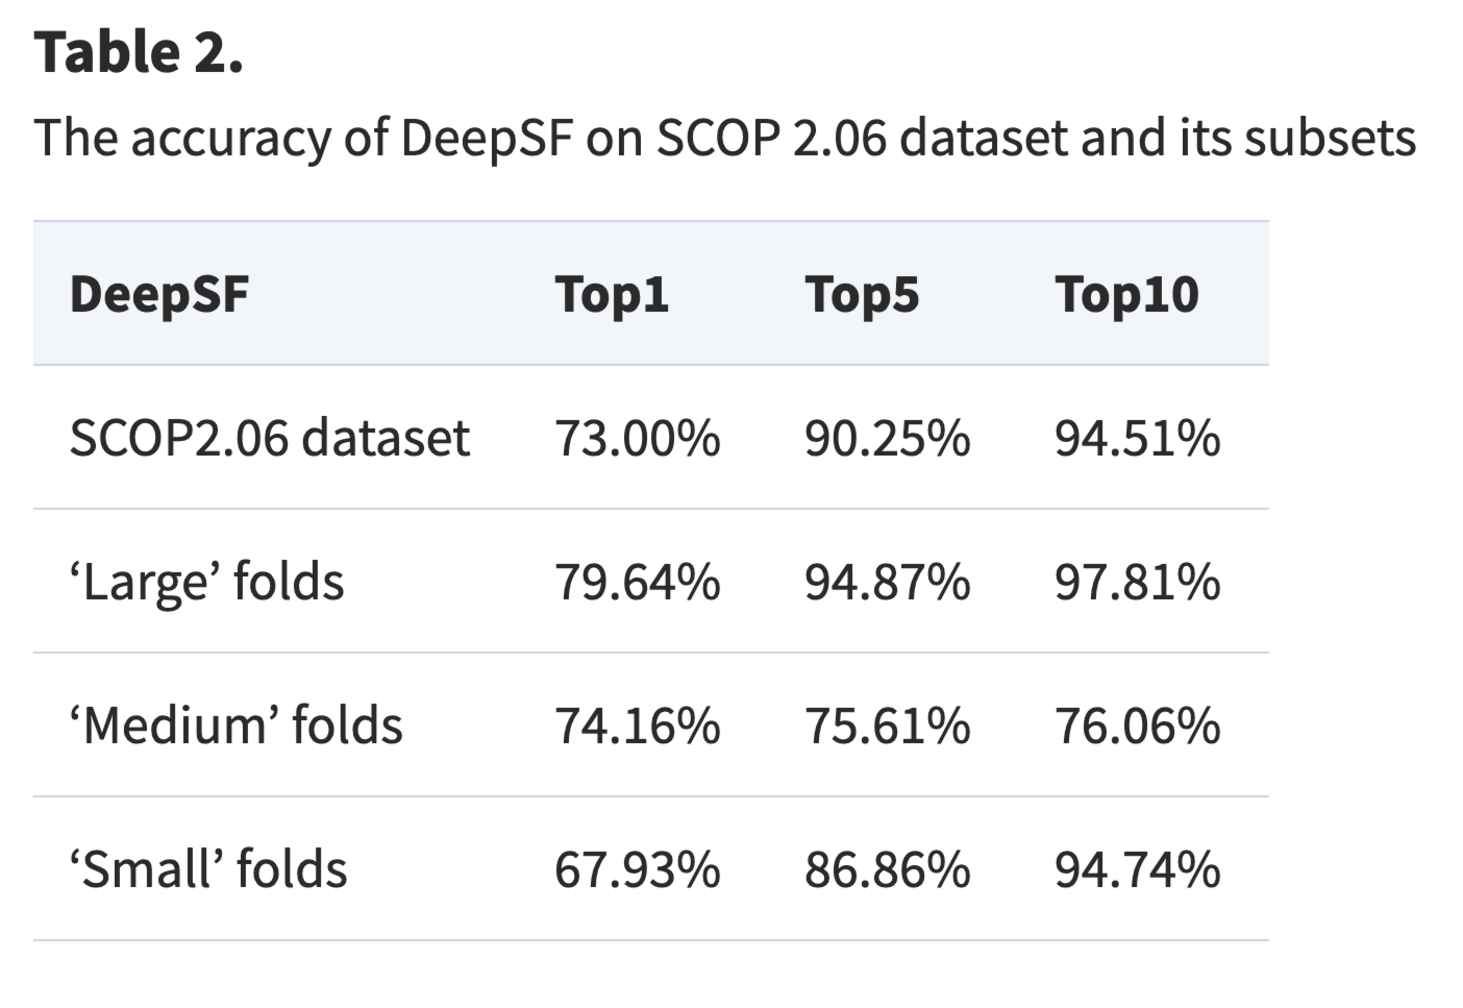
\includegraphics[height=2.5in]{./pics/table-2}
	%\caption{The prediction accuracy at family/superfamily/fold levels for top 1, top 5 and top 10 predictions of DeepSF and PSI-BLAST, on SCOP 1.75 test dataset}
	\label{fig:Table2}
	\end{figure}
}





%	Slide #3
\frame
{
	\frametitle{Experimental Results - 3}
	\framesubtitle{How do their proposed solutions compare with existing solutions?}


	\begin{figure}[h]
	\centering 
	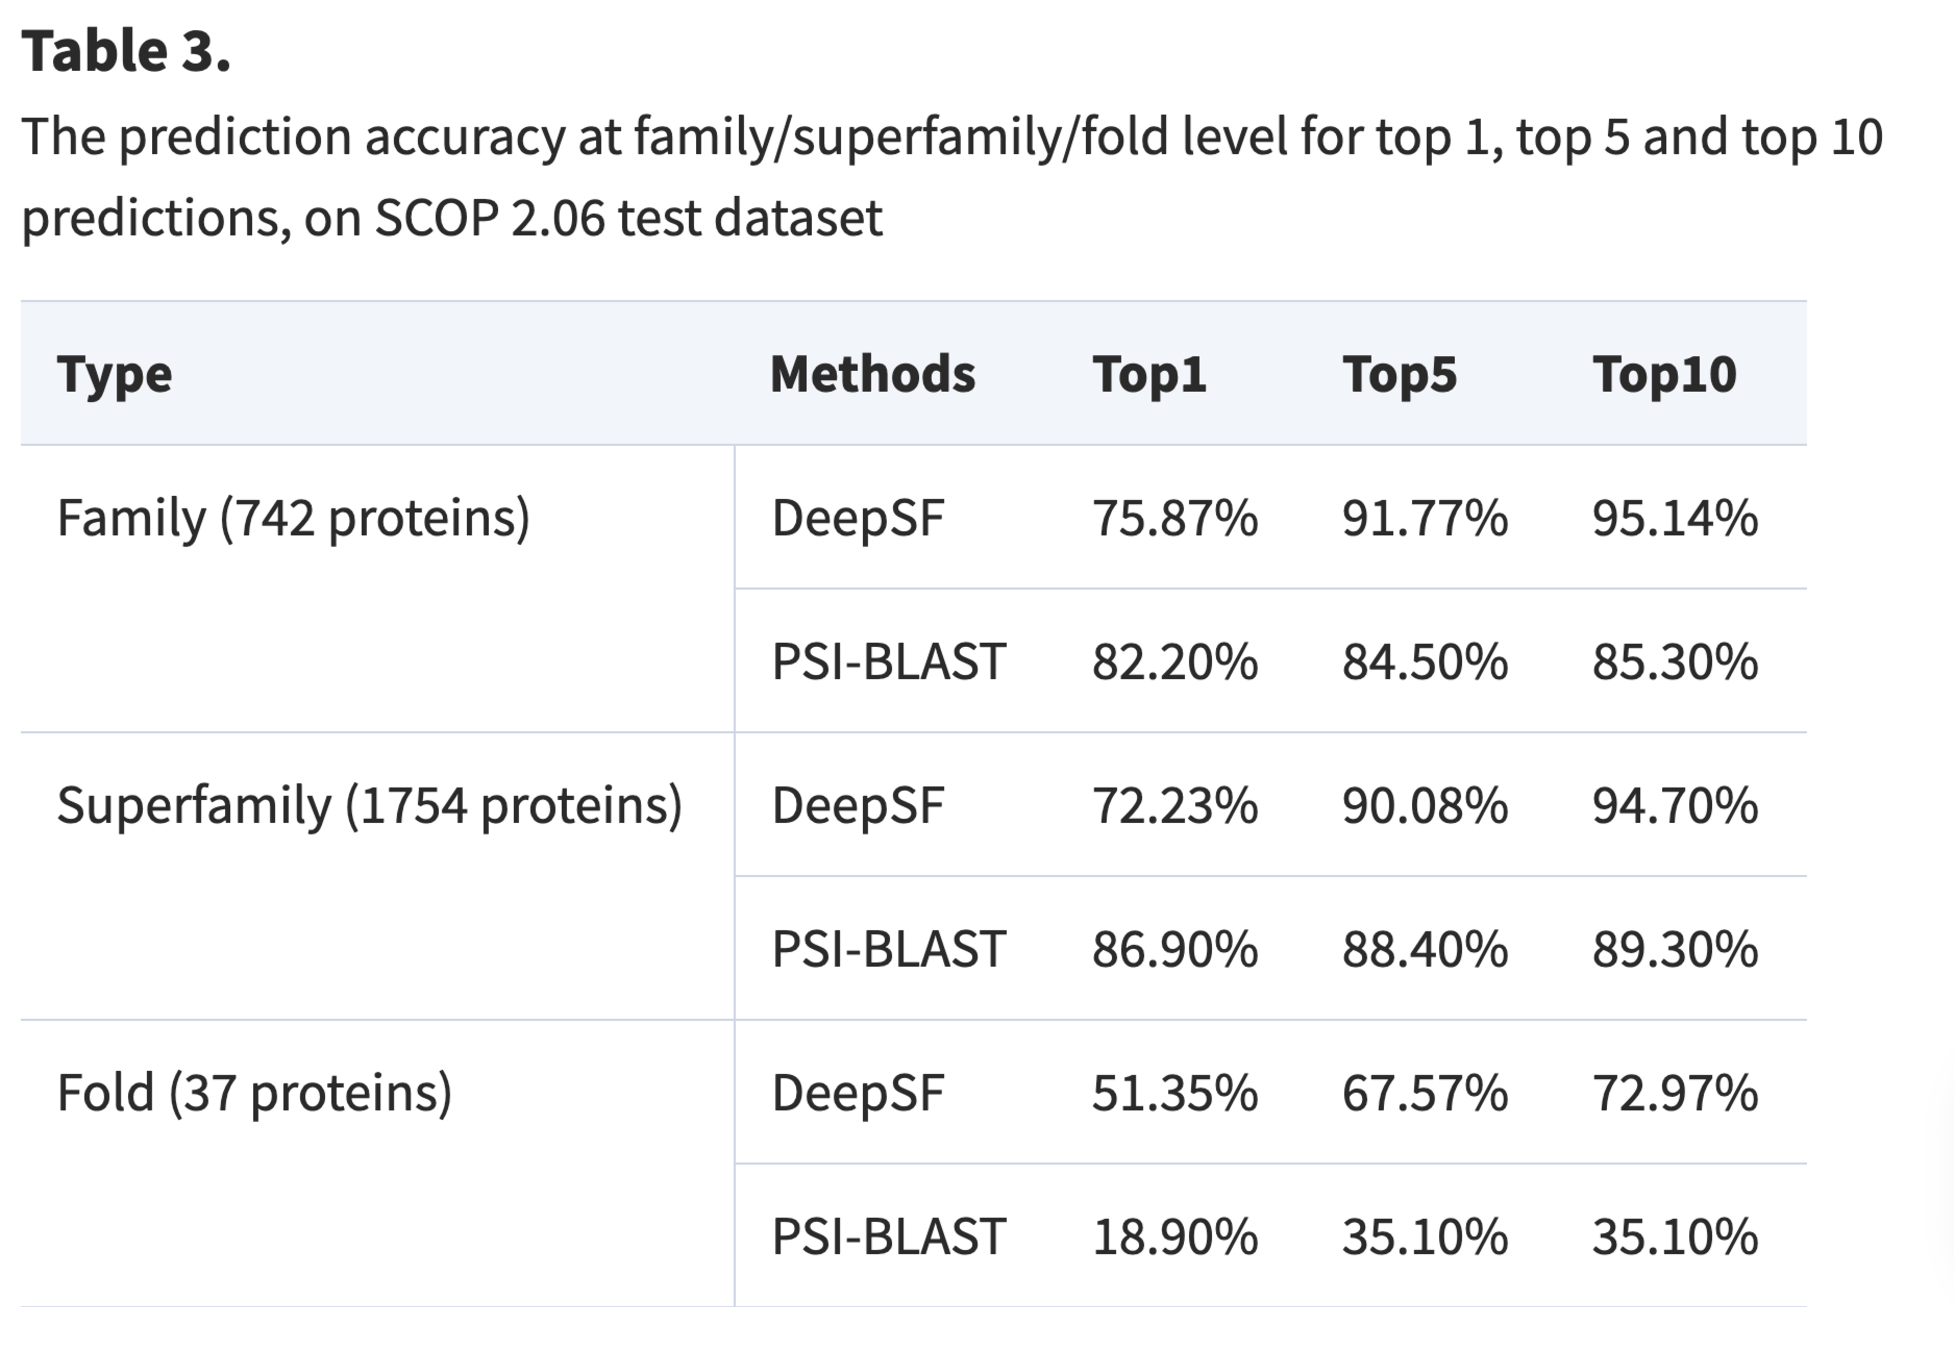
\includegraphics[height=2.5in]{./pics/table-3}
	%\caption{The prediction accuracy at family/superfamily/fold levels for top 1, top 5 and top 10 predictions of DeepSF and PSI-BLAST, on SCOP 1.75 test dataset}
	\label{fig:Table3}
	\end{figure}
}




%	Slide #4
\frame
{
	\frametitle{Experimental Results - 4}
	\framesubtitle{How do their proposed solutions compare with existing solutions?}


	\begin{figure}[h]
	\centering 
	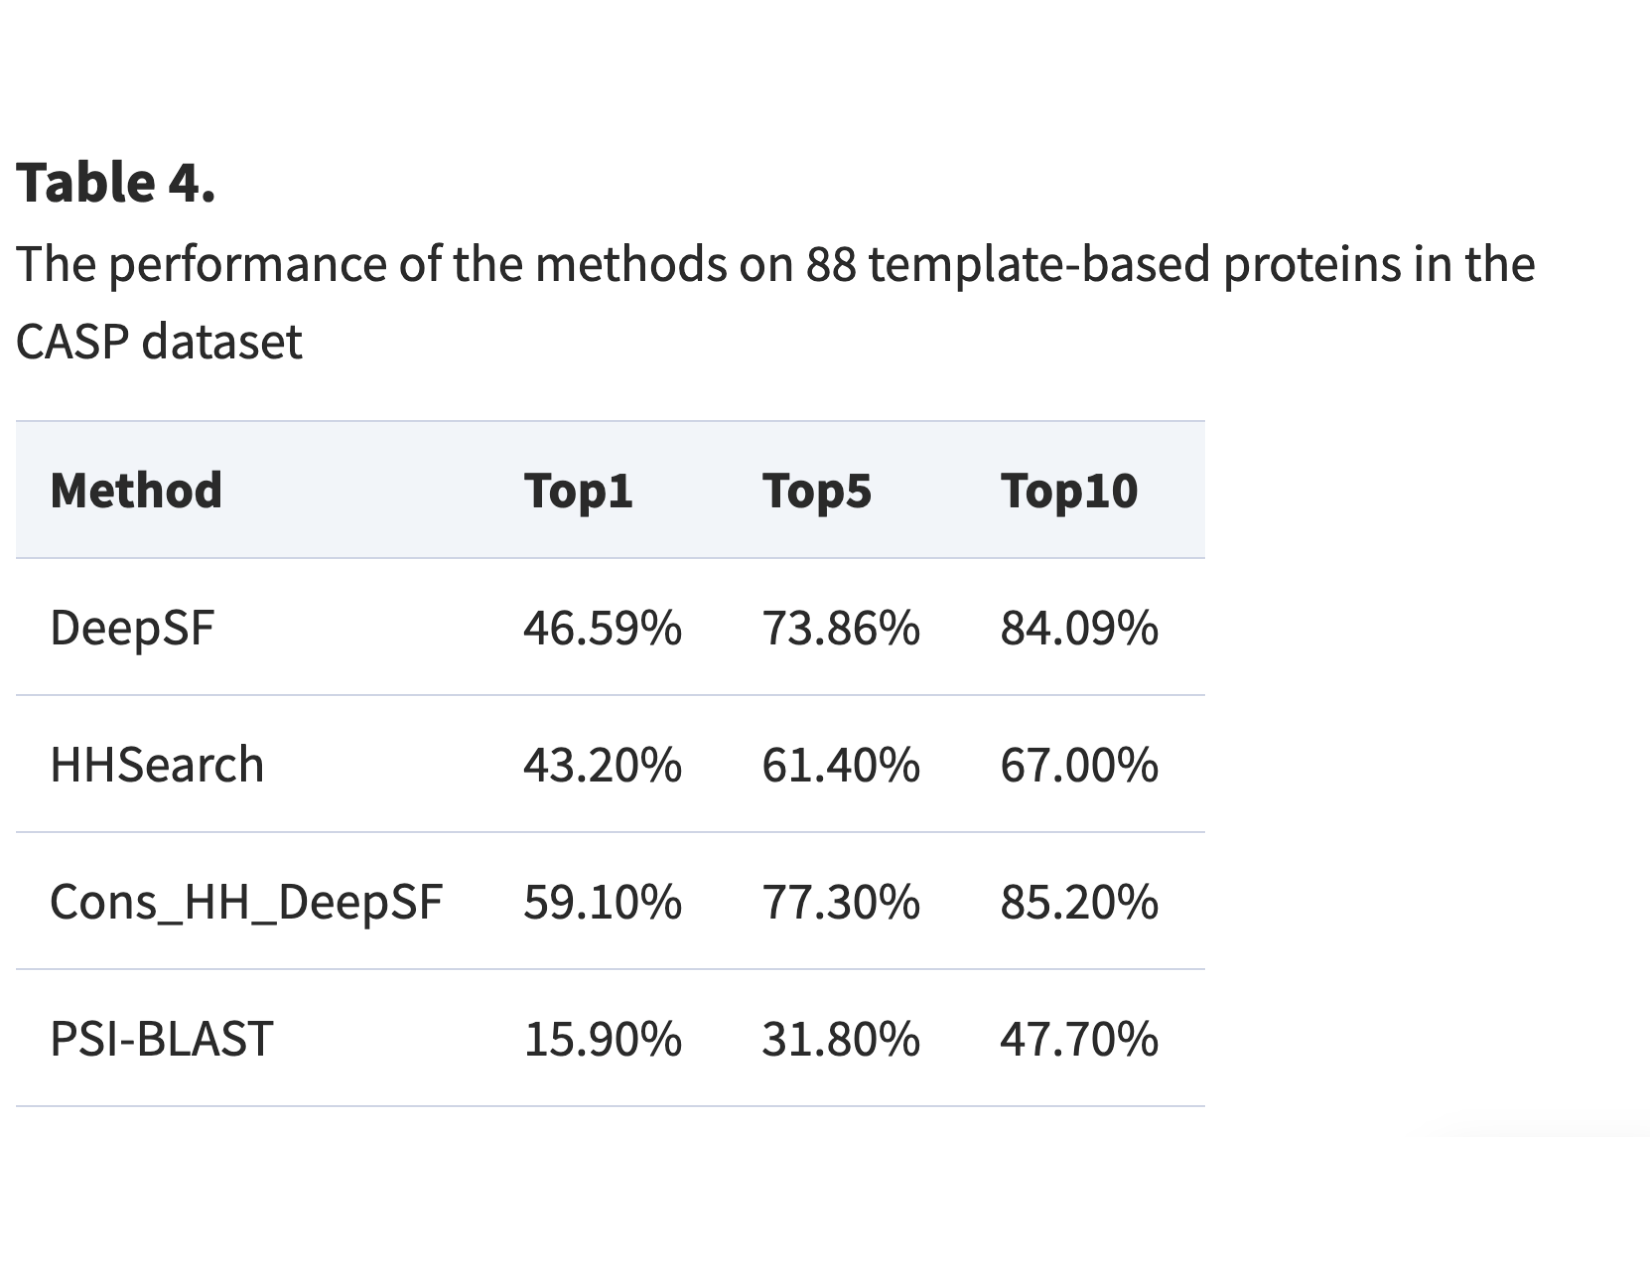
\includegraphics[height=2.5in]{./pics/table-4}
	%\caption{The prediction accuracy at family/superfamily/fold levels for top 1, top 5 and top 10 predictions of DeepSF and PSI-BLAST, on SCOP 1.75 test dataset}
	\label{fig:Table4}
	\end{figure}
}







%	Slide #5
\frame
{
	\frametitle{Experimental Results - 5}
	\framesubtitle{How do their proposed solutions compare with existing solutions?}


	\begin{figure}[h]
	\centering 
	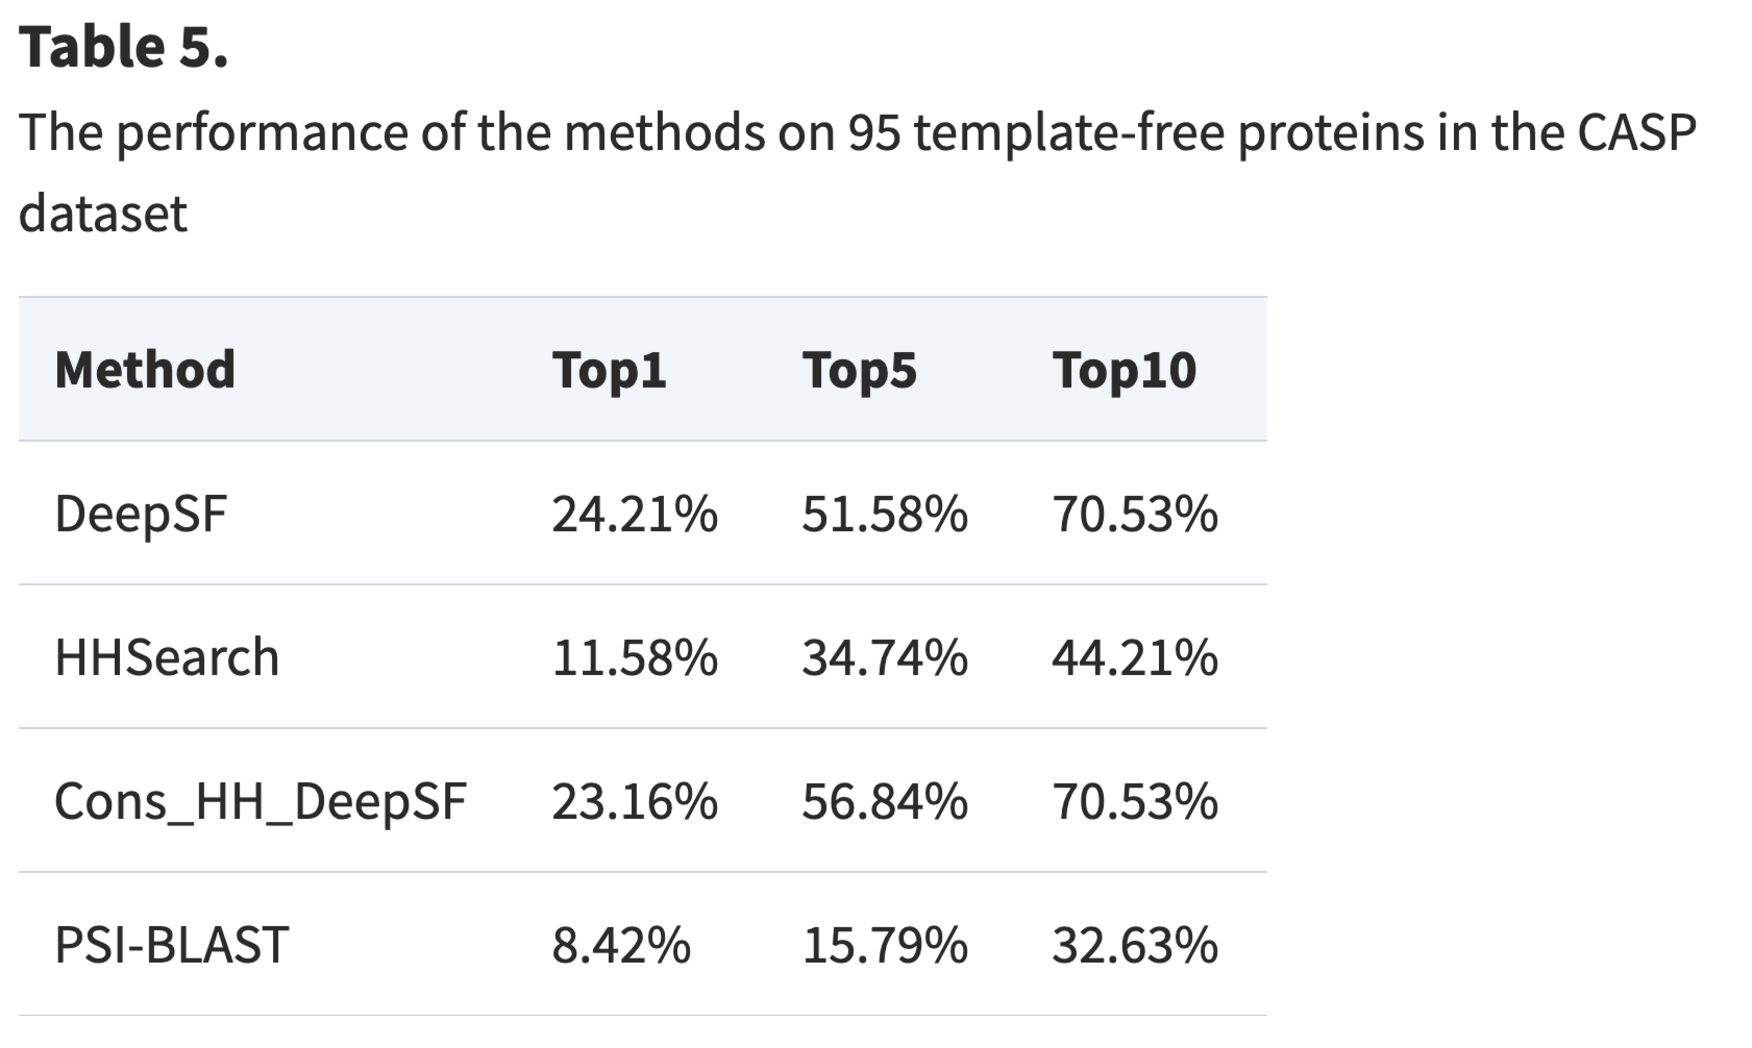
\includegraphics[height=2.5in]{./pics/table-5}
	%\caption{The prediction accuracy at family/superfamily/fold levels for top 1, top 5 and top 10 predictions of DeepSF and PSI-BLAST, on SCOP 1.75 test dataset}
	\label{fig:Table5}
	\end{figure}
}





%	Slide #6
\frame
{
	\frametitle{Experimental Results - 6}
	\framesubtitle{How do their proposed solutions compare with existing solutions?}


	\begin{figure}[h]
	\centering 
	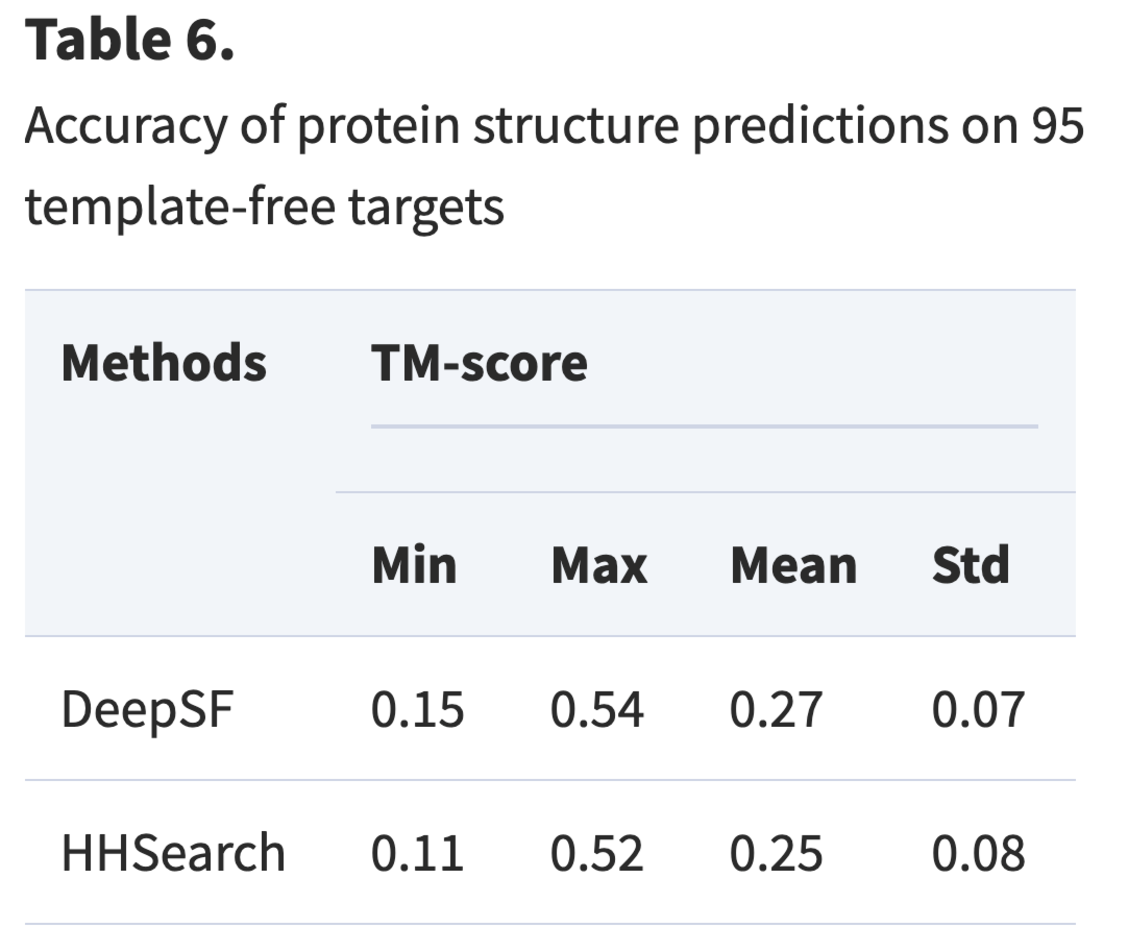
\includegraphics[height=2.5in]{./pics/table-6}
	%\caption{The prediction accuracy at family/superfamily/fold levels for top 1, top 5 and top 10 predictions of DeepSF and PSI-BLAST, on SCOP 1.75 test dataset}
	\label{fig:Table6}
	\end{figure}
}



























%	Slide #2
\frame
{
	\frametitle{Experimental Results - 2}
	\framesubtitle{How do their proposed solutions compare with existing solutions?}

	Experimental Results - 2.
	\begin{itemize}
	\item 
	\end{itemize}

}









%	Slide #3
\frame
{
	\frametitle{Experimental Results - 3}
	\framesubtitle{Benchmarking}

	Benchmarking of results with PSI-BLAST.
	\begin{itemize}
	\item Solution is 12.63-26.32\% better than HHSearch on template-free modeling targets.
	\item Solution is 3.39-17.09\% better on hard template-based modeling targets.
	\end{itemize}

}










%%%%%%%%%%%%%%%%%%%%%%%%%%%%%%%%%%%%%%%%%%%%%%
%	Discussion and Muddy Points

\section{Discussion and Muddy Points}


%	Slide #1
\frame
{
	\frametitle{Discussion of Experimental Results}
	\framesubtitle{What do the experimental results tell us?}

	Discuss the experimental results.
	\begin{itemize}
	\item Method is robust against: 
		\begin{enumerate} 
		\item sequence mutation
		\item insertion
		\item deletion
		\item truncation
		\end{enumerate}
	\item Can solve other protein pattern recognition problems:
		\begin{enumerate} 
		\item protein clustering
		\item protein comparison
		\item protein ranking
		\end{enumerate}
	\end{itemize}

}


%	Slide #2
\frame
{
	\frametitle{Weaknesses - 1}
	\framesubtitle{What are the weaknesses of this paper?}

	\begin{itemize}
	\item Poor benchmarking methodology: 
		\begin{enumerate} 
		\item Benchmarked solution (especially in Table 1) against PSI-BLAST (Altschul S.F. et al. , 1997)
		\item Did not benchmark with other modern solutions for protein fold prediction
			\begin{enumerate} 
			\item PFPA (2015, IEEE Transactions on NanoBioscience); DOI: 10.1109/TNB.2015.2450233
			\item random forest (2014, BMC Bioinformatics); DOI:10.1186/1471-2105-15-S11-S14
			\item PFP-RFSM (2013, J. Biomedical Science and Engineering); DOI:10.4236/jbise.2013.612145 
			\end{enumerate}
		\end{enumerate}
	\item Did not use box plots or bar charts to compare methods for each protein sequence in the datasets:
	\end{itemize}
}





%	Slide #3
\frame
{
	\frametitle{Weaknesses - 2}
	\framesubtitle{What are the weaknesses of this paper?}

	\begin{itemize}
	\item Inadequate \href{https://blog.apastyle.org/apastyle/tables-and-figures/}{cross-referencing of figures and tables} in the text: 
		%	https://gradschool.utah.edu/thesis/tables-and-figures/
		%	https://guides.lib.umich.edu/c.php?g=283073&p=1888264
		%	https://graduate.asu.edu/sites/default/files/chicago-quick-reference_0.pdf
		%	https://graduateschool.nd.edu/assets/283522/wfrw_ii_figures_and_tables.pdf
		%	https://www.overleaf.com/learn/latex/Cross_referencing_sections_and_equations
		%	https://guides.lib.monash.edu/citing-referencing/apa-tables-figures
		%	https://aso-resources.une.edu.au/academic-writing-course/information-basics/tables-figures/
		%	https://pressbooks.bccampus.ca/technicalwriting/chapter/figurestables/
		%	https://www.elsevier.com/__data/promis_misc/HPE_GfA.pdf
		%	http://www.maths.adelaide.edu.au/anthony.roberts/LaTeX/ltxxref.php
		%	https://en.wikipedia.org/wiki/Cross-reference
		\begin{enumerate} 
		\item When figures and tables are not cross referenced in the text, it takes more work to determine the context for each figure and table that I come across. The location of the figures and tables can be placed
		\item Did not benchmark with other modern solutions for protein fold prediction
			\begin{enumerate} 
			\item PFPA (2015, IEEE Transactions on NanoBioscience); DOI: 10.1109/TNB.2015.2450233
			\item random forest (2014, BMC Bioinformatics); DOI:10.1186/1471-2105-15-S11-S14
			\item PFP-RFSM (2013, J. Biomedical Science and Engineering); DOI:10.4236/jbise.2013.612145 
			\end{enumerate}
		\end{enumerate}
	\item Did not use box plots or bar charts to compare methods for each protein sequence in the datasets:
	\end{itemize}
}














%	Slide #3
\frame
{
	\frametitle{Muddy Points}
	\framesubtitle{What do I not understand about \cite{Hou2018}?}

	What do I not understand about \cite{Hou2018}?
	\begin{itemize}
	\item Why is it bad for top 1 predicted fold, but better for top 5 and top 10 predicted folds?
	\end{itemize}

}














%%%%%%%%%%%%%%%%%%%%%%%%%%%%%%%%%%%%%%%%%%%%%%
%\section{References}

\frame
{
	\frametitle{References}

%	\begin{itemize}
%	\item \cite{Weng2011}
%	\end{itemize}
%}


	{\linespread{1}
	%\bibliographystyle{IEEEtran}
	\bibliographystyle{plain}
	%%%%%%%\bibliography{/Users/zhiyang/Documents/ricerca/saag-bibtex/references}
	\bibliography{references}
	%\addcontentsline{toc}{chapter}{Bibliography}
	}
}





\end{document}


%
%	Trying to delay the not-uncommon path of engineering Ph.D.s who end up becoming "PowerPoint engineers"... Hopefully, slapping together a bunch of presentation slides to talk about any topic in any reasonable finite amount of time is not the most useful skill that I would learn as a grad student... Hey, at least I did it in LaTeX/Beamer!!!






 